\documentclass{beamer}\usepackage[]{graphicx}\usepackage[]{color}
%% maxwidth is the original width if it is less than linewidth
%% otherwise use linewidth (to make sure the graphics do not exceed the margin)
\makeatletter
\def\maxwidth{ %
  \ifdim\Gin@nat@width>\linewidth
    \linewidth
  \else
    \Gin@nat@width
  \fi
}
\makeatother

\definecolor{fgcolor}{rgb}{0.345, 0.345, 0.345}
\newcommand{\hlnum}[1]{\textcolor[rgb]{0.686,0.059,0.569}{#1}}%
\newcommand{\hlstr}[1]{\textcolor[rgb]{0.192,0.494,0.8}{#1}}%
\newcommand{\hlcom}[1]{\textcolor[rgb]{0.678,0.584,0.686}{\textit{#1}}}%
\newcommand{\hlopt}[1]{\textcolor[rgb]{0,0,0}{#1}}%
\newcommand{\hlstd}[1]{\textcolor[rgb]{0.345,0.345,0.345}{#1}}%
\newcommand{\hlkwa}[1]{\textcolor[rgb]{0.161,0.373,0.58}{\textbf{#1}}}%
\newcommand{\hlkwb}[1]{\textcolor[rgb]{0.69,0.353,0.396}{#1}}%
\newcommand{\hlkwc}[1]{\textcolor[rgb]{0.333,0.667,0.333}{#1}}%
\newcommand{\hlkwd}[1]{\textcolor[rgb]{0.737,0.353,0.396}{\textbf{#1}}}%
\let\hlipl\hlkwb

\usepackage{framed}
\makeatletter
\newenvironment{kframe}{%
 \def\at@end@of@kframe{}%
 \ifinner\ifhmode%
  \def\at@end@of@kframe{\end{minipage}}%
  \begin{minipage}{\columnwidth}%
 \fi\fi%
 \def\FrameCommand##1{\hskip\@totalleftmargin \hskip-\fboxsep
 \colorbox{shadecolor}{##1}\hskip-\fboxsep
     % There is no \\@totalrightmargin, so:
     \hskip-\linewidth \hskip-\@totalleftmargin \hskip\columnwidth}%
 \MakeFramed {\advance\hsize-\width
   \@totalleftmargin\z@ \linewidth\hsize
   \@setminipage}}%
 {\par\unskip\endMakeFramed%
 \at@end@of@kframe}
\makeatother

\definecolor{shadecolor}{rgb}{.97, .97, .97}
\definecolor{messagecolor}{rgb}{0, 0, 0}
\definecolor{warningcolor}{rgb}{1, 0, 1}
\definecolor{errorcolor}{rgb}{1, 0, 0}
\newenvironment{knitrout}{}{} % an empty environment to be redefined in TeX

\usepackage{alltt}
\usepackage{../371g-slides}
% Uncomment these lines to print notes pages
% \pgfpagesuselayout{4 on 1}[letterpaper,border shrink=5mm,landscape]
% \setbeameroption{show only notes}
\title{Probability Review 2}
\subtitle{Lecture 2}
\author{STA 371G}
\IfFileExists{upquote.sty}{\usepackage{upquote}}{}
\begin{document}
  
  

  \frame{\maketitle}

  % Show outline at beginning of each section
  \AtBeginSection[]{ 
    \begin{frame}<beamer>
      \tableofcontents[currentsection]
    \end{frame}
  }

  %%%%%%% Slides start here %%%%%%%

   \begin{darkframes}
  

	\begin{frame}[label=lists]{Sample vs Population}
    	Suppose you need to find out what the average house price in Austin is. How would you do that? 
    	% Assume that no one has done this before, so it is your duty.
    	
		\begin{figure} 
			\centering
			\scalebox{.4}{ 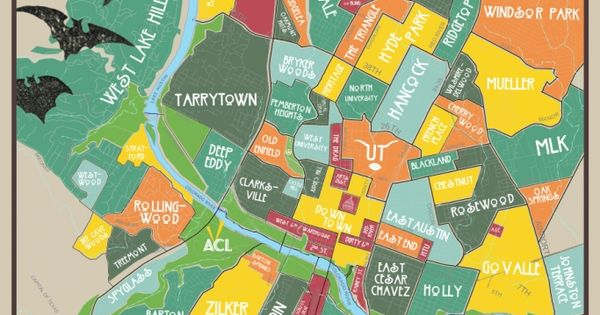
\includegraphics{austin.jpg} }
			\setlength\fboxsep{0pt}
			\setlength\fboxrule{0.5pt}
		\end{figure}  
			
		
		Planning to look into each house price? You better start now! 
		
		Because there are 360,000 houses in Austin!  
		
		Can we do something smarter? 
		
     
      
    \end{frame}    
    
    
    
    \begin{frame}[label=lists]{Sample vs Population}
    	A smarter approach would be to
   		\begin{itemize}
   			\item Pick $n$ houses randomly (e.g. $n=100$)
   			\item Take the average of the prices of these $n$ houses
   			\item Hope that average of your sample is close to the true price average.
   		\end{itemize}
   		
   		% Emphasize that the sample should be selected randomly to avoid any biases.
   		
		Just like doing polls to predict election results!
		
    \end{frame}    



    \begin{frame}[label=lists]{Sample vs Population}
    	Estimating a \alert{population parameter} (in this case mean) based on a \alert{sample statistic} (in this case, sample mean).
		
		\begin{itemize}
   			\item Population $\leftarrow$ all houses in Austin
			\item Sample $\leftarrow$  $n$ houses you picked
			\item Population mean $\leftarrow$ price average of all houses in Austin
			\item Sample mean $\leftarrow$ average price of $n$ houses in your sample 			
   		\end{itemize}
		
    	We could also estimate other population parameters, such as variance using the sample variance.
		
    \end{frame}  
 

    \begin{frame}[label=lists]{Collecting a sample}
    
    \begin{columns}[onlytextwidth]
        \column{.45\textwidth}
        	On Zillow.com, type ``Austin, TX.'' 
        	\begin{itemize}
   				\item Click ``More Map''
   				\item Select 15 houses, note their prices in an R script. 
   				\item Do not discard any price, use the first 15
   				\item Try to represent different regions
			\end{itemize}
        
         
        \column{.5\textwidth} 
        	
        	\begin{figure} 
				\centering
				\scalebox{.35}{ 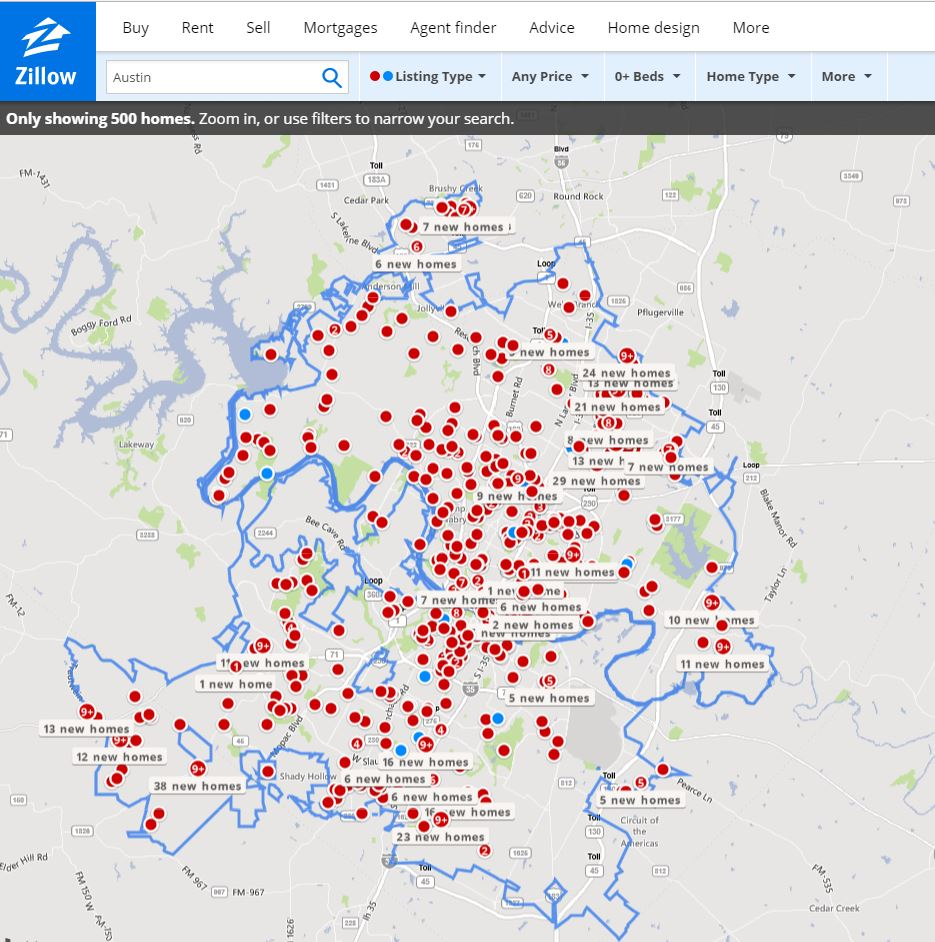
\includegraphics{zillow.jpg} }
				\setlength\fboxsep{0pt}
				\setlength\fboxrule{0.5pt} 
			\end{figure} 	
        	        
        \end{columns}
					
    \end{frame}  
    
    
    
    
    	\defverbatim[colored]\sampleZillow{
      \begin{lstlisting}[language=R,tabsize=2]
# Create a vector of house prices (You should have 15 price data)
sample_house_prices <- c(327000,276000,513000)
# Calculate sample statistics
sample_mean <- mean(sample_house_prices)
sample_variance <- var(sample_house_prices)
sample_standard_deviation <- sd(sample_house_prices)
# Sample mean of first 5 houses
sample_mean_5 <- mean(sample_house_prices[1:5])
# Print them to console
cat("Sample Mean", sample_mean)
cat("Sample Variance", sample_variance)
cat("Sample Standard Deviation", sample_standard_deviation)
cat("Sample Mean of first 5 houses",sample_mean_5)

    \end{lstlisting}}	
    
    \begin{frame}[label=lists]{Collecting a sample}
    Your R script should look like this
    \sampleZillow
    
    \end{frame}


    \begin{frame}[label=lists]{Sampling Distribution} 
		On Learning Catalytics, enter your results. \newline
		
		We will plot their histogram later.		
    \end{frame}



    \begin{frame}[label=lists]{Sampling Distribution}
    	Everyone found a different sample mean, which one is correct?
    	None. \newline %But they should be all clustered around the true mean (the average house price in Austin). \newline
    	
    	Sample mean (your answers) itself has a distribution, separate from the house price distribution in Austin. This is called  \alert{sampling distribution}. \newline
    	
    	Expected value of the sample mean $=$ Population mean
    	
    	Standard deviation of the sample mean ($s$) $=$ Standard deviation of the population ($\sigma$) / $\sqrt{n}$ \newline
    	
    	The higher the sample size ($n$), the lower the standard deviation of the sample mean ($s$).
		
    \end{frame}
    
    
    
    \begin{frame}[label=lists]{Sampling Distribution}
    
    Assume the average house price in Austin ($\mu$) is \$300K and the standard deviation $\sigma=$\$60K. (You don't know these!) \newline
    
    (Assuming normal distribution), 99.7\% of the houses are between \$$[120K, 480K]$. \newline
    
    Sample mean's mean \$$300$K, standard deviation \$$60K/\sqrt{n}$. \newline
    
    $n=25$ houses, $s=60K/5=12K$, 99.7\% of surveys in \$$[274K, 336K]$.
    
	$n=100$ houses, $s=60K/10=6K$, 99.7\% of surveys \$$[282K, 318K]$.
    
    \end{frame}
    
    
    \begin{frame}[label=lists]{Sampling Distribution}
		Let's compare sample mean of 5 houses vs 15 houses. \newline
		
		What do you expect to see?
	\end{frame}	
	
	\begin{frame}[label=lists]{Sampling Distribution}
		\begin{figure} 
				\centering
				\scalebox{.5}{ 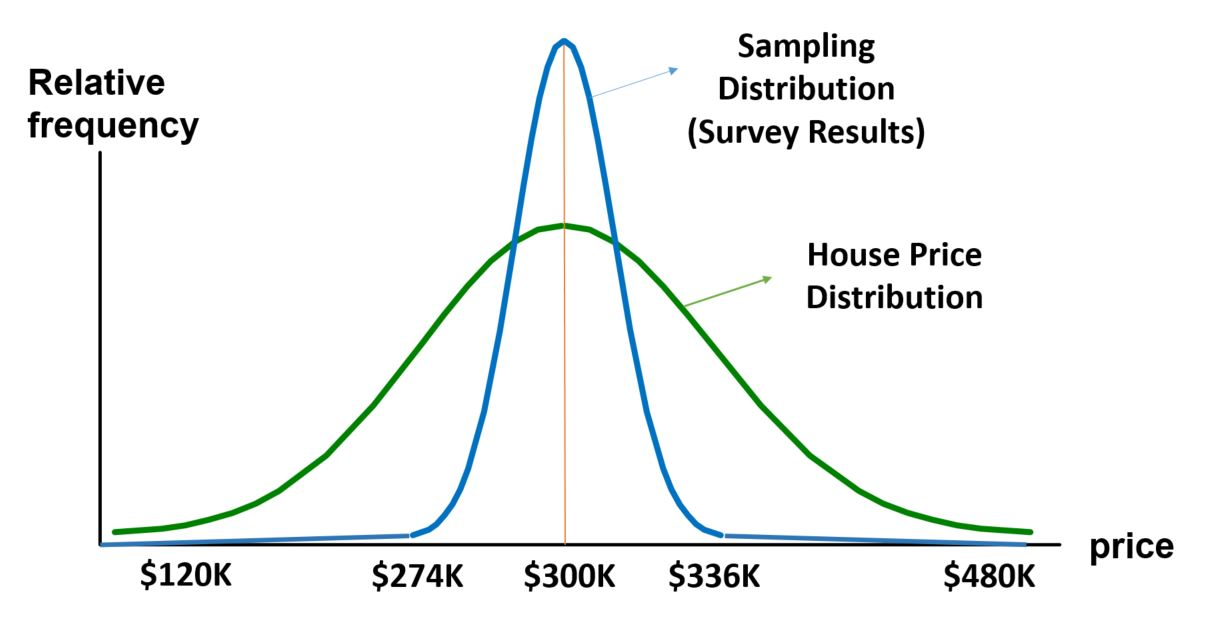
\includegraphics{sampling2.jpg} }
				\setlength\fboxsep{0pt}
				\setlength\fboxrule{0.5pt} 
			\end{figure} 	
	\end{frame}	
    
    
    \begin{frame}[label=lists]{$t$ Distribution}
		When population is normally distributed with $\mu$ and $\sigma^2$, sample mean has a normal distribution mean $\mu$ and variance $\sigma^2/n$. \newline
		
		If we don't know $\sigma$ (we often don't!), how can we use sample mean's distribution? \newline
		
		We use sample variance ($s$) instead. In that case, the sample mean will (after normalization) have a $t$ distribution.
	\end{frame}	
    
    
    
    \begin{frame}[label=lists]{Hypothesis Testing}
    Hypothesis: The average house price in Austin is \$1M.
    
    Your survey on 30 houses: Average price is \$$305K$. \newline
    
    Questions, questions...
    \begin{itemize}
   \item Would you reject the hypothesis? Why?
    
   \item Is it possible that, out of bad luck, you picked the cheapest houses?
    
   \item Would you be more comfortable with your conclusion if you had 1000 houses in your survey?
    
   \item When should you reject the hypothesis? When not?
    
   \end{itemize}


	\end{frame}
	
	
	\begin{frame}[label=lists]{P-Value}
		$H_0:$ $\mu=\$1M$	(Null hypothesis)
		
		$H_1:$ $\mu<\$1M$	(Alternative hypothesis)
		
		Assume that your sample mean is \$305K. \newline
		
		The \alert{$P$-value} is ``the probability of observing such an extreme (\$305K or less) sample statistic given the null hypothesis is true.''
		
		\begin{itemize}
		\item $P$-value  $\leq \alpha$, reject the null hypothesis
		\item $P$-value  $> \alpha$, reject the null hypothesis
		
		\end{itemize}	
		
		$\alpha$ is usually chosen as $0.05$ \underline{prior to sampling}.		
		
		% Ask how n would affect p value
		% Emphasize that the interpretation of p value is always the same.

	\end{frame}
	
	
	\begin{frame}[label=lists]{P-Value}
		Consider the null hypothesis true with $\mu=\$1M$ and $\sigma=\$200K$. For $n=25$, the sampling distribution has a mean $\$1M$ and the standard deviation $\$40000$. \newline
		
		Approximately 95\% of the surveys will give a result in \$$[920K, 1080K]$. \newline
		
		In fact, P-value of a sample mean of \$305K is $5\times 10^{-143}$. \newline
		
		Rather than thinking you are cursed, you simply reject the hypothesis!
	\end{frame}
	
	
		\begin{frame}[label=lists]{P-Value}
			\begin{figure} 
				\centering
				\scalebox{.5}{ 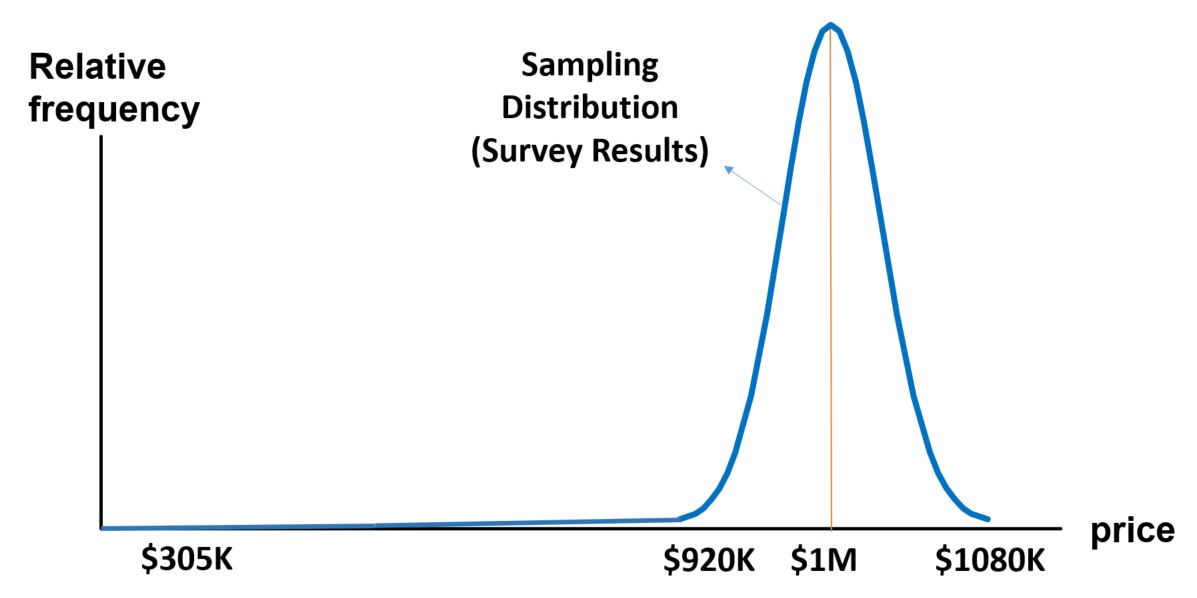
\includegraphics{pval.jpg} }
				\setlength\fboxsep{0pt}
				\setlength\fboxrule{0.5pt} 
			\end{figure} 	
	\end{frame}
	
	

	
	\begin{frame}[label=lists]{Confidence Interval}
		Content Here
	\end{frame}
	
	
	\begin{frame}[label=lists]{Confidence Interval 2}
		Content Here
	\end{frame} 
	

\end{darkframes}
  
  
  

\end{document}

